\begin{bx1}
  薄く,平らで導電性の半径$R$の円形のディスクがその中心を$xy$平面の原点と
  一致させて存在しており,そのポテンシャルは$V$に保たれている.
  一定のポテンシャルをもつディスクの電荷密度が$(R^2 - \rho^2)^{-1/2}$に
  比例するとする.ただし,$\rho$は原点からはかったディスク上の距離である.
  このとき,
  \begin{enumerate}[(a)]%  
    \item $r > R$におけるポテンシャルが
      \begin{gather}%
        \Phi(r, \theta, \phi) = \frac{2V}{\pi} \frac{R}{r} \sum_{l=0}^\infty \frac{(-1)^l}{2l+1} \ab(\frac R r)^{2l} P_{2l}(\cos\theta)
      \end{gather}%
      で表されることを示せ.
    \item $r < R$におけるポテンシャルを決定せよ.
    \item ディスクのキャパシタンス(静電容量)はいくらか?
  \end{enumerate}%
\end{bx1}
\itemlabel{(a)}
  空間内の電荷分布は
  \begin{gather}%
    \rho_{\mr{c}}(\bs{x}) = \frac{a}{\sqrt{R^2-\rho^2}} H(R-\rho) \delta(z)
  \end{gather}%
  [ただし$H(\cdot)$はHeavisideのstep functionである]とかけるので,$a$を決定する.
  原点でのポテンシャルは
  \begin{gather}%
    V(0) = \frac{1}{4\pi \eps_0} \int \frac{1}{\rho'}\rho_{\mr{c}}(\bs{x'}) 
    \rho'\dl{\rho'} \dl{\phi'} \dl{z'}
    = \frac{\pi a}{4\eps_0}
  \end{gather}%
  と表されるので,$V(0) = V$として,電荷分布は
  \begin{gather}%
    \rho_{\mr{c}}(\bs{x}) = \frac{4\eps_0 V}{\pi} \frac{1}{\sqrt{R^2 - \rho^2}} 
    H(R-\rho) \delta(z)
  \end{gather}%
  である.
  これより,$z$軸上でのポテンシャルを計算することができて,
  \begin{align}%
    \Phi(z) &= \frac{1}{4\pi \eps_0} \int 
    \frac{\rho_{\mr{c}}(\bs{x'})}{\sqrt{(\rho')^2+z^2}} 
    \rho' \dl{\rho',\phi',z'}\notag\\
    &=\frac{2V}{\pi} \int_0^R \frac{\rho' \dl{\rho'}}
    {\sqrt{
      ((\rho')^2+z^2) (R^2-(\rho')^2)
    }}\notag\\
    &= \frac{2V}{\pi} \int_0^{\pi/2} 
    \frac{R\sin\theta\dl{\theta}}{\sqrt{z^2 + R^2\sin\theta}}\notag\\
    &= \frac{2V}{\pi} \arctan\ab(\frac{R}{|z|})
  \end{align}%
  と表すことができる[式\eqref{eq:3.676}を利用].

  $R / |z| \leq 1$とすると,
  \begin{gather}%
    \Phi(z) = \frac{2V}{\pi} \sum_{k=0}^\infty \frac{(-1)^k}{2k+1} \ab(\frac{R}{|z|})^{2k+1}
  \end{gather}%
  として級数展開することができるので,$R / r \leq 1$かつ$z \geq 0$のdisk上部では
  \begin{gather}%
    \Phi(\bs{x}) = 
    \frac{2V}{\pi}\sum_{l=0}^\infty \frac{(-1)^l}{2l+1} \ab(\frac{R}{r})^{2l+1}
    P_{2l}(\cos\theta)
  \end{gather}%
  と表される.$z \leq 0$のdisk%
  \footnote{diskとdiscは技術的な文脈では使い分けがあるらしい.
  discはCDやDVDなどの光学式メディアを指し,diskはフロッピーディスクやハードディスク
  などを指すらしい.}
  下部では$z=0$面に関してポテンシャルが対称である
  として,
  \begin{align}%  
    \Phi(\bs{x}) & = \frac{2V}{\pi}\sum_{l=0}^\infty \frac{(-1)^l}{2l+1} \ab(\frac{R}{r})^{2l+1}
    P_{2l}(\cos(\pi-\theta))\\
    &= 
    \frac{2V}{\pi}\sum_{l=0}^\infty \frac{(-1)^l}{2l+1} \ab(\frac{R}{r})^{2l+1}
    P_{2l}(\cos\theta)
  \end{align}%
  となる.

\itemlabel{(b)}
  一方$R / |z| \geq 1$とすると,
  $\arctan(x) + \arctan(1/x) = \pi/2$に注意して,
  \begin{align}%
    \Phi(z) &= \frac{2V}{\pi}\ab[\frac{\pi}{2}-\arctan\ab(\frac{|z|}{R})]\notag\\
    &= V - \frac{2V}{\pi} \sum_{l=0}^\infty \frac{(-1)^l}{2l+1}\ab(\frac{|z|}{R})^{2l+1}
  \end{align}%
  であるから,
  $z \gtrless 0$では
  \begin{align}%
    \Phi(\bs{x}) &=
    \begin{dcases}
      V - \frac{2V}{\pi} \sum_{l=0}^\infty \frac{(-1)^l}{2l+1} \ab(\frac rR)^{2l+1} P_{2l+1}(\cos\theta)\\
      V - \frac{2V}{\pi} \sum_{l=0}^\infty \frac{(-1)^l}{2l+1} \ab(\frac rR)^{2l+1} P_{2l+1}(\cos(\pi-\theta))
    \end{dcases}\notag\\
    &= V \mp \frac{2V}{\pi}
    \sum_{l=0}^\infty \frac{(-1)^l}{2l+1} \ab(\frac rR)^{2l+1} P_{2l+1}(\cos\theta)
  \end{align}
  となる.

\itemlabel{(c)}
  導体上の全電荷は
  \begin{gather}%
    Q \equiv \int_0^R 2\pi \rho \dl{\rho} 
    \frac{4\eps_0 V}{\pi} \frac{1}{\sqrt{R^2  -\rho^2}} = 8\eps_0 VR
  \end{gather}%
  であるから,capacitanceは$C = Q/V = 8\eps_0 R$
  である.
  \begin{figure}[htbp]%  
    \centering%  
    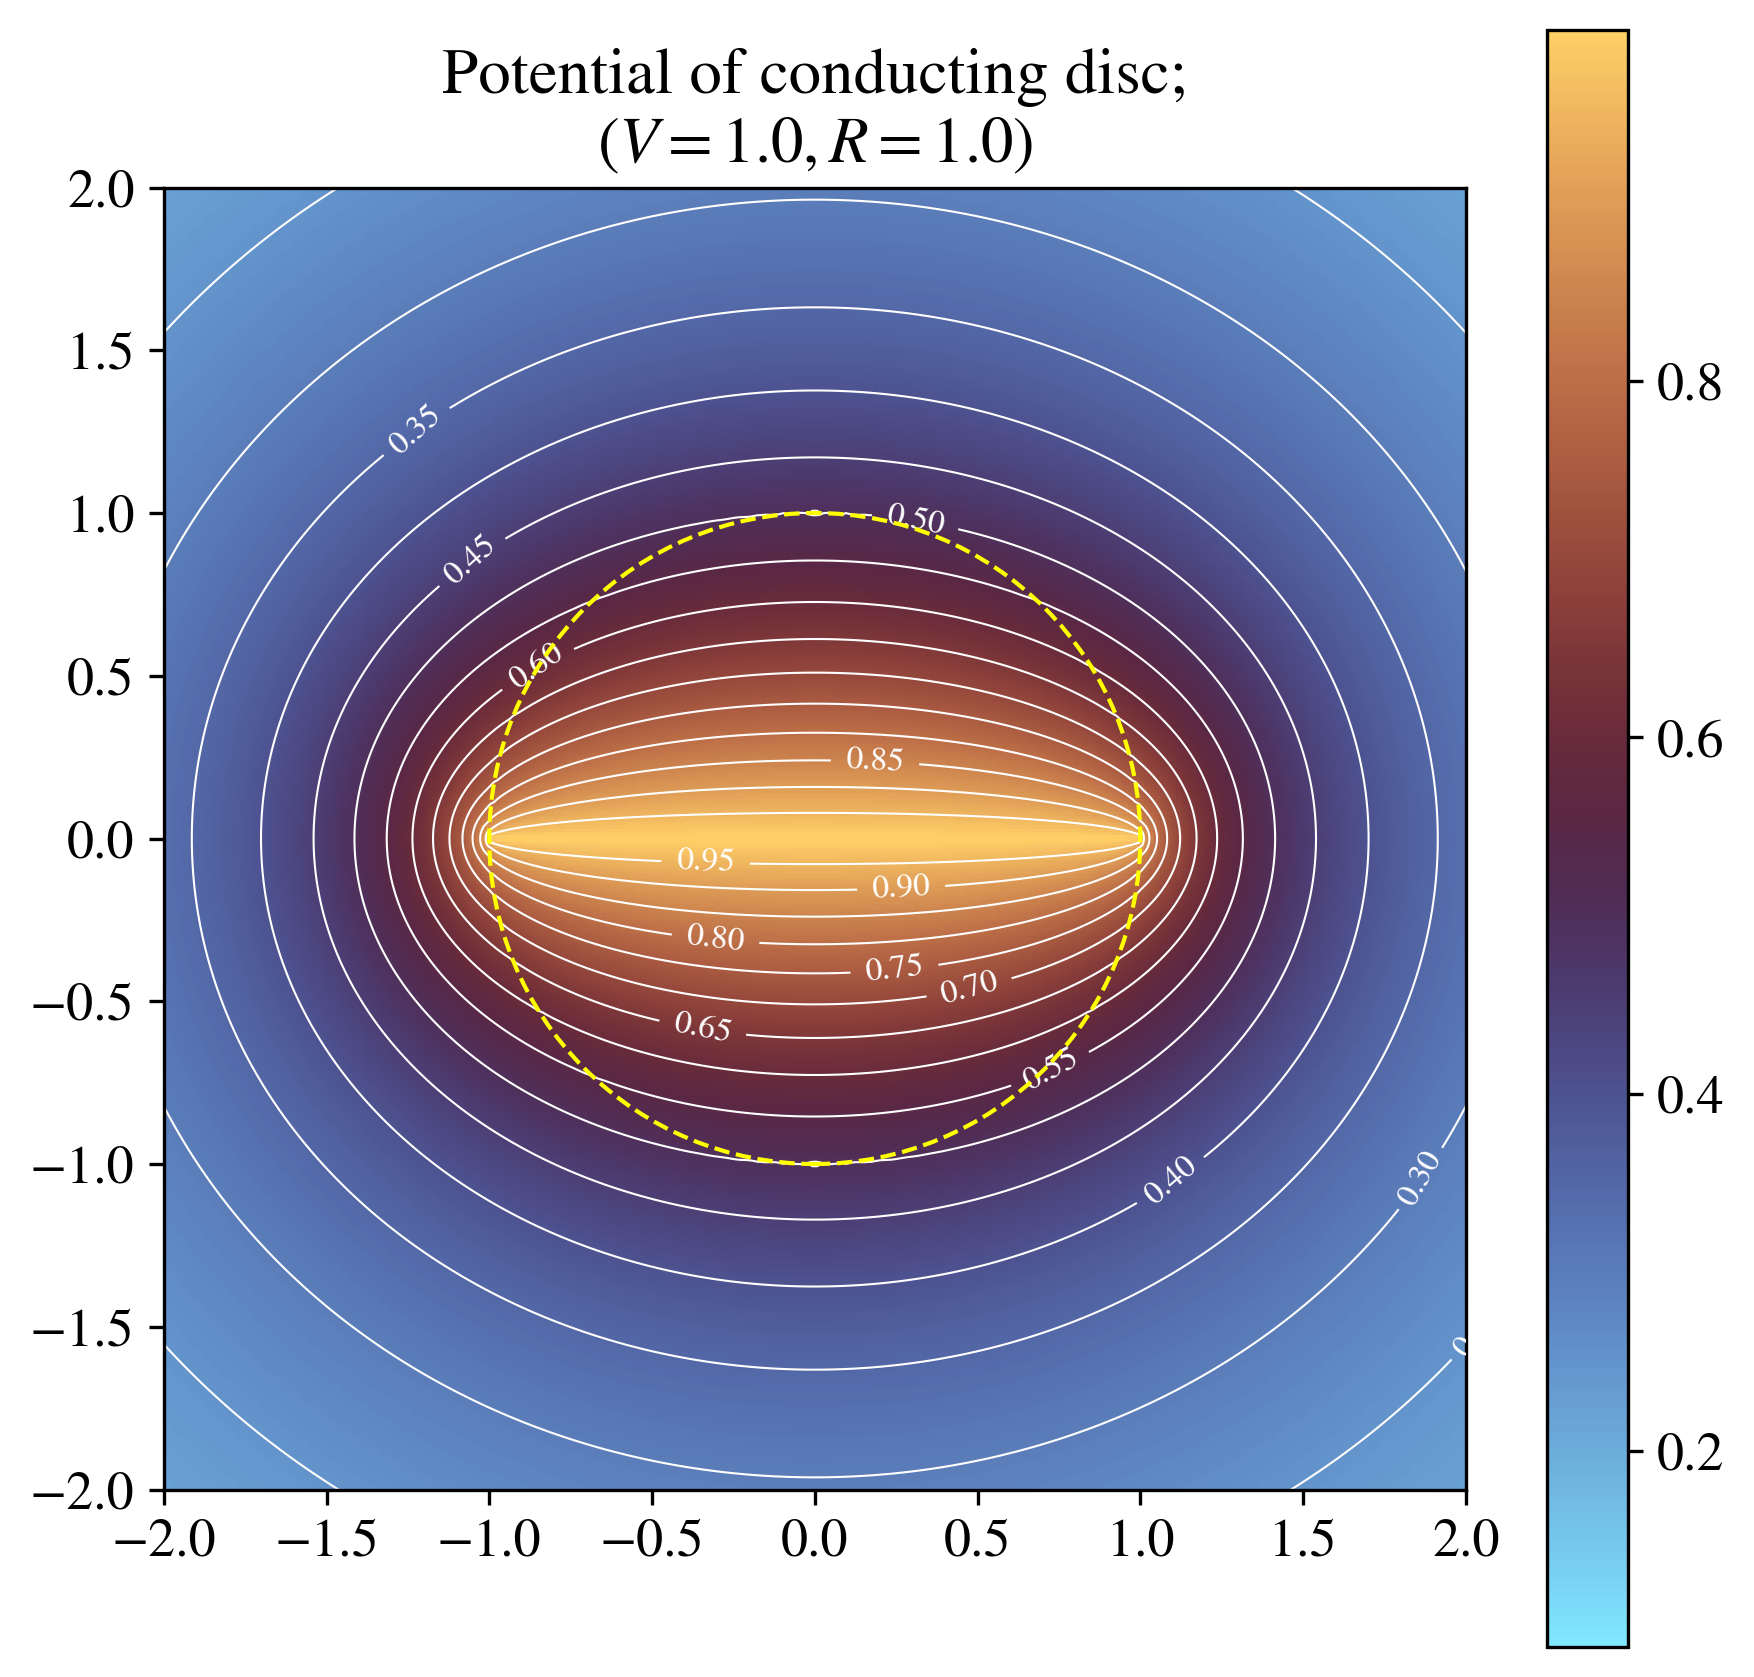
\includegraphics[width=0.5\linewidth]{py/3-3_normal_w_circle.png}%  
    \caption{$V=1.0$,$R = 1.0$として等ポテンシャル面を描画した図;
    ポテンシャルが$V$に保たれているdiskは$z$軸上の$-1 < x <1$の範囲である.
    また,図中の黄色破線は$r = R$となる球面を表しており,この面を境にして
    ポテンシャルの表式が変化している.}%  
    \label{fig:3-3_normal_w_circle}%  
  \end{figure}%

  \clearpage
